
\documentclass[a4paper,11pt]{article}

\usepackage{graphicx}
\usepackage{hyperref}         
\usepackage[english,UKenglish]{babel}
\usepackage{sistyle}
\usepackage{enumitem}

\usepackage{amsmath,amssymb}% AMS standards
\usepackage[adobe-utopia]{mathdesign}
\usepackage{fontspec,xltxtra,xunicode}

\defaultfontfeatures{Mapping=tex-text}

\renewcommand{\rmdefault}{Minion Pro}
\setmainfont[Mapping=tex-text,Numbers=Lowercase]{Minion Pro}
\setromanfont[Mapping=tex-text]{Minion Pro}
\setsansfont[Mapping=tex-text,Scale=MatchLowercase, Color=6C6C6C]{Myriad Pro}
\setmonofont[Scale=MatchLowercase]{Andale Mono}

\newcommand{\mtdefault}{\rmdefault}
\usepackage[medium,sf]{titlesec}   
\hbadness=10000
\hfuzz=50pt
\setcounter{totalnumber}{50}
\setcounter{topnumber}{50}
\setcounter{bottomnumber}{50}    
\usepackage[margin=3cm,bottom=3cm,nohead]{geometry}


\input{../symbols.tex}
\author{Baptiste Augui\'e}
\title{Fresnel formul\ae}      
 
\begin{document}
\maketitle

\section{Single interface}

Let us consider the situation depicted in figure~\ref{fig:interface}, 
% 
\begin{figure}[!ht]
\centering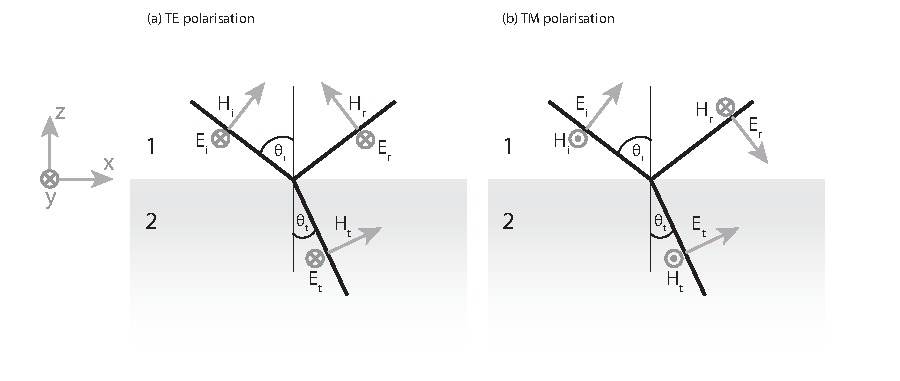
\includegraphics{interface}
\label{fig:interface}
\caption[Schematic of reflection and transmission by a single interface.]{Schematic of reflection and transmission by a single interface. Note that the orientation of the vectors has been chosen so as to have a  consistent picture at normal incidence.}
\end{figure}
% 
where we define the Fresnel coefficients as the ratio of the complex \emph{amplitude} of the \emph{electric} fields, $r= E_r/E_i$ for the reflection coefficient, and $t= E_t/E_i$ for the transmission coefficient. The Fresnel coefficients can be obtained by considering the continuity of the tangential component of the $E$ and $H$ fields at the interface. The continuity of the normal components of $D$ and $B$ does not yield supplementary conditions and will not be considered. It is worth noting that the continuity of $H^y$ is only valid for materials that do not sustain a surface current resulting from the addition of external charges. 

\subsection{TE-polarised light} % (fold)
\label{sub:te_polarised_light}
For TE-polarised light, the continuity of $E^y$ reads,
\[
E_i + E_r  = E_t
\]
which yields,
\begin{equation}
	1+r =t.
\label{eq:rt1}
\end{equation}
The continuity of $H^y$ can be written as,
\[
H_i\cos\theta_i - H_r\cos\theta_i  = H_t\cos\theta_t
\]
It is convenient to express the angles in terms of the normal component of the $k$-vectors,
\begin{equation}
	k_z = n k_0 \cos\theta.
\label{eq:k}
\end{equation}
for the incident, reflected, and refracted fields, so that $\cos\theta_t / \cos\theta_i=\dfrac{k_{z2}n_1}{k_{z1}n_2}$. The complex magnitude of the magnetic and electric fields are linked in each medium by the optical impedance. Its expression can be obtained from the induction law,
\[
\nabla\times \bE = -\partial_t \bB
\]
expressed in Fourier space\footnote{assuming here a homogeneous plane wave} as,
\[
\bk\times \bE = i\omega \bB
\]
The ratio $E/H$ is the impedance, written as,
\begin{equation}
	\frac{E}{H}= c \mu \mu_0 / n= \sqrt{\frac{\mu\mu_0}{\veps\veps_0}}=Z\cdot Z_0.
\label{eq:impedance}
\end{equation}
We can define the admittance $Y$ as the inverse impedance, $Y=\dfrac{1}{Z\cdot Z_0}$
Using \ref{eq:k} and \ref{eq:impedance}, the continuity of $H^y$ can be expressed as,
\[
Y_1 (1 - r) =  Y_2 \frac{n_1k_{z2}}{n_2k_{z1}}t.
\]
After rearranging, we obtain,
\begin{equation}
	1 - r = \frac{\mu_1k_{z2}}{\mu_2k_{z1}}t.
\label{eq:rt2}
\end{equation}
We can summarize the two continuity relations in the following system,

\begin{equation*} \left\{
\begin{aligned}
1 + r &= t\\
1 - r &= \frac{\mu_1k_{z2}}{\mu_2k_{z1}}t
\end{aligned}\right.
\end{equation*}
Solving for $r$ and $t$ yields the result,
\begin{equation} 
t_{12}^s=\frac{2\mu_2 k_{z1}}{\mu_2 k_{z1}+\mu_1k_{z2}},\qquad r_{12}^s=\frac{\mu_2 k_{z1}-\mu_1k_{z2}}{\mu_2 k_{z1}+\mu_1k_{z2}}.
\label{eq:fresnels}
\end{equation}

\subsection{TM-polarised light} % (fold)
\label{sub:tm_polarised_light}
For TM-polarised light, the continuity of $H^y$ reads,
\[
Y_1 (1 - r) = Y_2 t
\]
rewritten as,
\begin{equation}
	1 - r =\sqrt{\frac{\mu_1\veps_2}{\mu_2\veps_1}}\cdot t.
\label{eq:rt3}
\end{equation}
Note that in the case of normal incidence, we can combine equation~\ref{eq:rt1} and equation~\ref{eq:rt3}, 
\[
t_{12} = \frac{2\sqrt{\mu_2\veps_1}}{\sqrt{\mu_2\veps_1}+\sqrt{\mu_1\veps_2}}, \qquad r_{12}=\frac{\sqrt{\mu_2\veps_1}-\sqrt{\mu_1\veps_2}}{\sqrt{\mu_1\veps_2}+\sqrt{\mu_2\veps_1}}.
\]
The continuity of $E^y$ can be written,
\[
E_i\cos\theta_i + E_r\cos\theta_i  = E_t\cos\theta_t
\]
and can be expressed in terms of the normal component of the wave-vectors as,
\[
1 + r = \frac{n_1k_{z2}}{n_2k_{z1}}t.
\]

We can summarize the two continuity relations in the following system,

\begin{equation*} \left\{
\begin{aligned}
1 - r &=\sqrt{\frac{\mu_1\veps_2}{\mu_2\veps_1}}t\\
1 + r &=\frac{n_1k_{z2}}{n_2k_{z1}}t
\end{aligned}\right.
\end{equation*}
% 
Solving for $r$ and $t$ yields the result,
\begin{equation} 
t_{12}^p=\frac{2\varepsilon_2 k_{z1}}{\varepsilon_2 k_{z1}+\varepsilon_1k_{z2}}\sqrt{\frac{\mu_2\varepsilon_1}{\mu_1\varepsilon_2}},\qquad r_{12}^p=\frac{\varepsilon_2 k_{z1}-\varepsilon_1k_{z2}}{\varepsilon_2 k_{z1}+\varepsilon_1k_{z2}}.
\label{eq:fresnelp}
\end{equation}

To summarize, for a single interface from 1 to 2 with normal along the $z$ direction, the Fresnel coefficients read,
	% 
	\begin{equation} 
	\begin{aligned}
	r_{12}^p&=\frac{\varepsilon_2 k_{z1}-\varepsilon_1k_{z2}}{\varepsilon_2 k_{z1}+\varepsilon_1k_{z2}},&{}& r_{12}^s&=\frac{\mu_2 k_{z1}-\mu_1k_{z2}}{\mu_2 k_{z1}+\mu_1k_{z2}}\\
	t_{12}^p&=\frac{2\varepsilon_2 k_{z1}}{\varepsilon_2 k_{z1}+\varepsilon_1k_{z2}}\sqrt{\frac{\mu_2\varepsilon_1}{\mu_1\varepsilon_2}},&{}& t_{12}^s&=\frac{2\mu_2 k_{z1}}{\mu_2 k_{z1}+\mu_1k_{z2}}.
	\end{aligned}
	\label{eq:fresnel}
	\end{equation}

Note that,
\begin{equation}
	r_{ij}=-r_{ji}.
\label{eq:t}
\end{equation}
To verify the conservation of energy, one must consider the irradiance defined in terms of the electric field as $I=\addfontfeature{Fractions=On}\text{1⁄2}Y|E|^2$, yielding,
\begin{equation}
	R=\frac{I_r}{I_i}=|r|^2, \qquad T=\frac{I_t}{I_i}=\frac{Y_1}{Y_2}|t|^2.
\label{eq:irradiance}
\end{equation}
and we can verify that, indeed, $R+T=1$ for a single interface.
% subsection tm_polarised_light (end)

\section{Reflectivity of a layer} % (fold)
\label{sec:two_interfaces}
% 
From the viewpoint of ray optics, a thin layer will support an infinite number of internal reflections (absorption and irregularities will however reduce the intensity in a physical situation). The infinite series of reflected orders can be expressed in the form a geometric sum, leading to a closed form formula as shown below.
	\begin{figure}[!ht]
	\centering	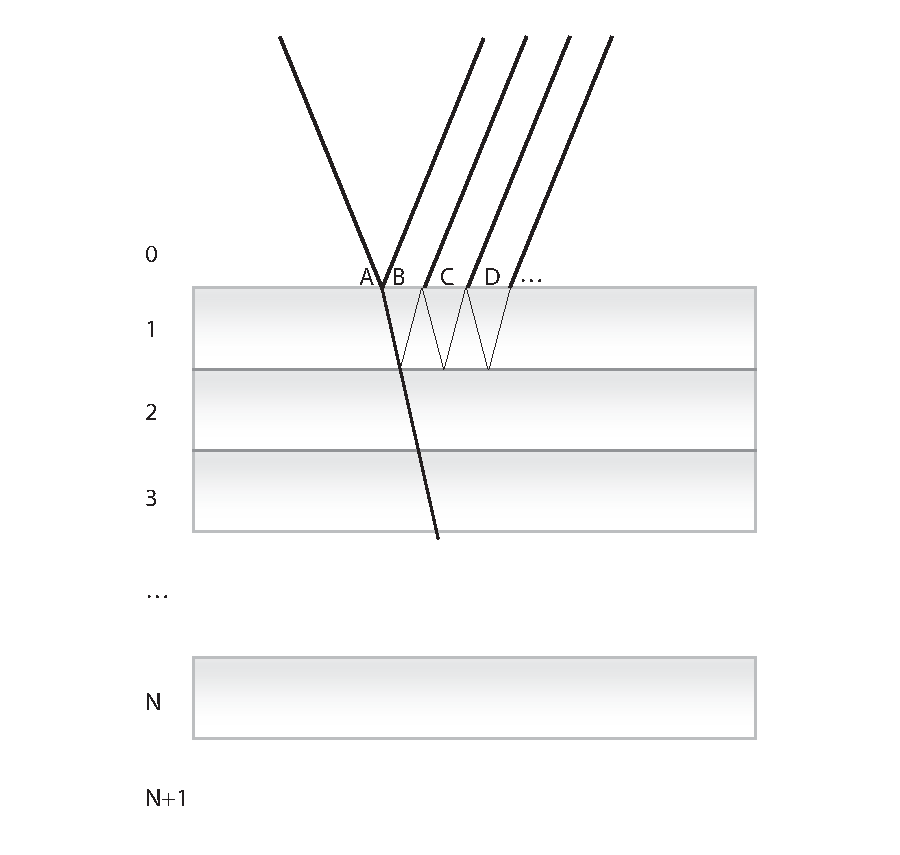
\includegraphics{stack}
	\label{fig:fresnel}
	\caption[Schematic of reflection and transmission by a multilayer stack.]{Schematic of reflection and transmission by a multilayer stack. A few reflected orders are noted `A', `B', `C' and `D' for the first film.}
	\end{figure}
An incident plane wave with amplitude $A$ impinges on the first interface. It can be reflected, $B=r_{01}A$, or transmitted. The total response of the slab can be obtained by following each order of reflection inside the slab (`C', `D', \dots).

Upon transmission at the first interface, the wave amplitude is $t_{01}A$. Application of Fermat's principle yields a phase change $\Delta \phi= k_{z1}d$ when the wave hits the second interface. The reflection coefficient at this interface is $r_{12}$. The partial wave reflected from this path, noted `C', is therefore $C=t_{10}t_{01}r_{12}\exp(2i k_{z1}d)A$.

Similarly, in `D', \[
	D=t_{10}t_{01}r_{10}r_{12}^2\exp(4i k_{z1}d)A
	\]
And, for the ${j^\text{th}}$ partial wave,
	\[
	t_{10}t_{01}r_{12}^{j}r_{10}^{{j-1}}\exp(2i {j}k_{z1}d)A
	\]
The wave reflected by the slab is the sum of these contributions,
	\[
	r_{\text{slab}}A=B+C+D+\dots=\left[r_{01}+t_{10}t_{01}r_{12}\sum_{j=0}^{\infty}r_{12}^jr_{10}^{j}\exp(2ji k_{z1} d)\right]A
	\]
For clarity, I write $\beta=r_{12}r_{10}\exp(2i k_{z1}d)$. The summation of all partial waves is thereby expressed as a geometrical sum,
	\[
	r_{\text{slab}}=r_{01} + \left(t_{10}t_{01}r_{12}\exp(2i k_{z1}d)\right)\sum_{j=0}^{\infty}\beta^j
	\]
Recalling that the sum of a geometric series of common ratio $q$ is $\frac{1}{1-q}$, we can write,
	\[
	r_{\text{slab}}=r_{01} + \frac{t_{10}t_{01}r_{12}\exp(2i k_{z1}d)}{1-r_{12}r_{10}\exp(2i k_{z1}d)}
	\]

We note from equations~\ref{eq:rt1} and~\ref{eq:rt3} and the relation $r_{ij} = -r_{ji}$ that for either polarisation we have the following identity,
\begin{equation}
	t^s_{ij}t^s_{ji}  = (1-r^s_{ij})(1+r^s_{ij})= 1-(r^s_{ij})^2 ,\qquad 
	t^p_{ij}t^p_{ji}  =\frac{Y_i}{Y_j}(1-r^p_{ij})\frac{Y_j}{Y_i}(1+r^p_{ij}) = 1-(r^p_{ij})^2
\label{eq:identity}
\end{equation}
Using equation~\ref{eq:identity} and the substitution $r_{10} = -r_{01}$ we finally obtain,
	\begin{equation}
		r_{\text{slab}}=\frac{r_{01}+r_{12}\exp(2i k_{z1}d)}{1+r_{01}r_{12}\exp(2i k_{z1}d)}.
	\label{eq:fresnelSlab}
	\end{equation}

For the transmission, one obtains,

	\begin{equation}
		t_{\text{slab}}=\frac{t_{01}t_{12}\exp(i k_{z1}d)}{1+r_{01}r_{12}\exp(2i k_{z1}d)}.
	\label{eq:fresnelTSlab}
	\end{equation}

% section two_interfaces (end)

When N layers are stacked together, the reflection coefficient of the structure can be found by applying recursively the preceding formula for a single layer. This amounts to considering one of the reflection coefficients to be the effective reflection accounting for all the layers behind.


\end{document}